\documentclass[cn]{elegantbook}
\usepackage[square,numbers,sort&compress]{natbib}
\newcommand{\upcite}[1]{\textsuperscript{\textsuperscript{\cite{#1}}}}

\tikzstyle{startstop} = [rectangle, rounded corners, minimum width = 2cm, minimum height=1cm,text centered, draw = black, fill = red!40]
\tikzstyle{arrow} = [->,>=stealth]

% title info
\title{模式识别作业1}
\subtitle{基于模板匹配的手写数字识别}
% bio info
\author{罗雁天}
\institute{清华大学电子系}
\version{2018310742}
\date{\today}
\logo{logo.png}
\cover{cover.jpg}

\begin{document}

\maketitle
\tableofcontents
\mainmatter
\hypersetup{pageanchor=true}
% add preface chapter here if needed
\chapter{问题描述}
本次作业使用模板匹配的方法来对手写数字字符进行识别。提供两组数据,分别存放在train文件夹和test文件夹中.
\begin{itemize}
	\item train文件夹中存放已单独分割出来的0-9数字图像模板,模板已统一到相同的尺度,每个模板为对应的数字外切分割结果;
	\item test文件夹中有8张用于测试的图像,其中6张正常尺度(与模板尺度相同),一张存在划痕,一张有噪声。
\end{itemize}

本次作业便利用此给出的图像模板对测试图像进行数字字符识别。
\section{模板图像预处理}
为了获得更好的识别效果和识别的鲁棒性,我们对训练集中的8张图片进行预处理,这里主要采用的算法便是将其二值化。我们将二值化后的图像保存到单独的文件夹中,方便我们之后进行模板匹配的操作。图\ref{res1}显示了训练集模板图片预处理前后的对比图,上面部分为训练集的原始灰度图片,下面图片为预处理之后的二值化图片。

\begin{figure}[!h]
	\centering
	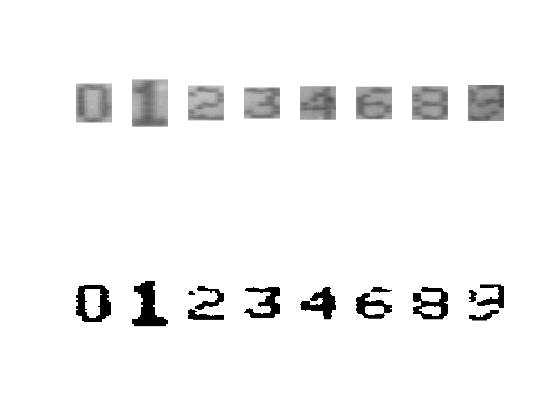
\includegraphics[width=0.8\textwidth]{res1}
	\caption{\label{res1}训练集数据预处理前后对比图}
\end{figure}

\section{测试集噪声图片预处理}
\label{sec12}
对于含有噪声的图片,如果我们直接对其进行二值化,可以看出噪声很多,直接识别的话效果不佳,如图\ref{res2}所示。因此我们首先对其进行维纳滤波,如图\ref{res2}所示,可以看出维纳滤波可以较好的滤除了噪声。但是如果维纳滤波之后的图片直接进行二值化,可以看出左侧数字部分相比于直接二值化有了较大提升,但是右侧较暗的区域依然不足以识别。因此我们需要对其进行背景均衡化处理,具体算法为:

\begin{itemize}
	\item 首先对图像进行模糊滤波得到背景图;
	\item 定义全局亮度为整张图片的亮度平均值;
	\item 计算$I_{balance}=I-background(I)+\bar{I}$
\end{itemize}
从图\ref{res2}最后的结果看出,使用此种算法处理之后的二值化图片具有较好的直观效果。

\begin{figure}[!h]
	\centering
	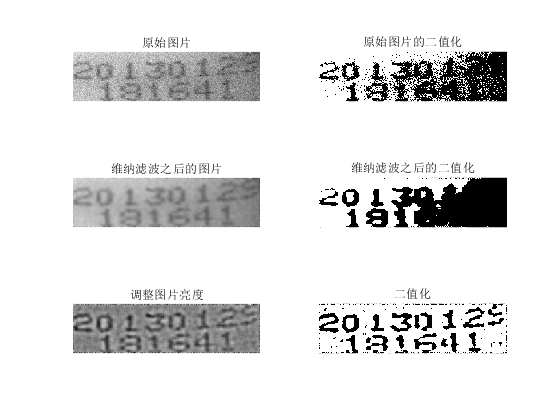
\includegraphics[width=\textwidth]{res2}
	\caption{\label{res2}噪声图片预处理对比图}
\end{figure}

\section{测试集划痕图片预处理}
\label{sec13}
如图\ref{res3}所示,划痕图片中划痕的灰度值明显较小,因此我们可以设置一个阈值(在本实验中设置为90),将灰度值小于90的直接置为缺失值,得到中间图所示的情况,可以看出划痕部分已经完全检测出来了。然后我们使用插值的算法填充缺失值即可得到下面图所示的结果,从中可以看出,使用此算法可以较好的去除划痕。

\begin{figure}[!h]
	\centering
	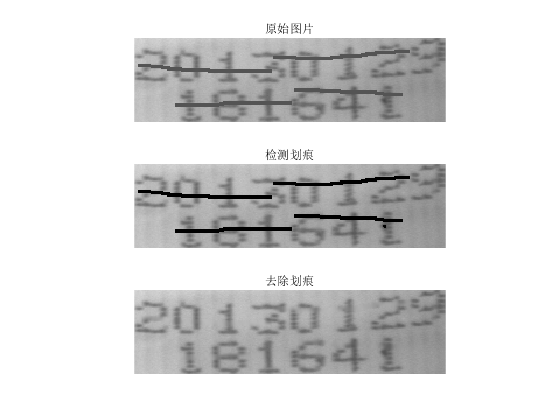
\includegraphics[width=\textwidth]{res3}
	\caption{\label{res3}划痕图片预处理对比图}
\end{figure}

\chapter{简单模板匹配}
可以用扫描窗的方式对测试图像进行扫描,每个扫描窗进行模板匹配,若最接近某个模板,就认为是该模板对应的数字。同时也需注意拒识非数字字符的窗口。同时观察测试图片发现可以对其进行分割,使得分割之后的每一块都包含一个数字字符,然后与模板进行匹配,认为匹配度高的便是该模板对应的数字。本章节对以上两种方法都进行尝试,并给出识别的结果。并且在test文件夹中还有两张进行过放缩处理的图片,对其我们便不能直接使用滑窗对其进行判别,因此我们对其使用多尺度扫描的方式进行检测。

\section{基于分割的模板匹配}
\label{sec1}
观察测试集的图片可以看出每一张测试图片都有多个数字组成,我们首先可以对齐进行分割,分割成小的图像块,然后对每一个图像块进行裁剪、二值化的预处理之后与预处理之后的训练集进行模板匹配操作,得到匹配值最大的数便认为是识别出来的字符。对于平均灰度值超过一定阈值(在本实验中设置为0.95)的图像块,便认为该图像块没有数字。

\subsection{正常图片识别结果}
对6张正常图片进行识别,识别输出一个$2\times 8$的矩阵,矩阵每一个元素代表该图像块识别出来的数字字符,inf代表该图像块没有数字。识别结果如图\ref{res4}所示。

\begin{figure}[!h]
	\centering
	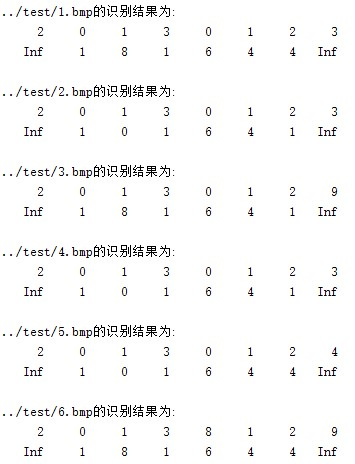
\includegraphics[width=\textwidth]{res4}
	\caption{\label{res4}正常图片识别结果}
\end{figure}

\subsection{噪声图片识别结果}
首先对噪声图片进行第\ref{sec12}节介绍的预处理操作,然后再对其进行模板匹配操作,得到如图\ref{res5}所示的识别结果。

\begin{figure}[!h]
	\centering
	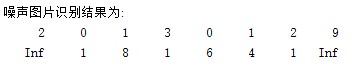
\includegraphics[width=\textwidth]{res5}
	\caption{\label{res5}噪声图片识别结果}
\end{figure}

\subsection{划痕图片识别结果}
首先对划痕图片进行第\ref{sec13}节介绍的预处理操作,然后再对其进行模板匹配操作,得到如图\ref{res6}所示的识别结果。

\begin{figure}[!h]
	\centering
	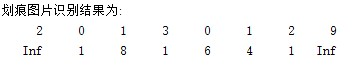
\includegraphics[width=\textwidth]{res6}
	\caption{\label{res6}划痕图片识别结果}
\end{figure}

\subsection{结果总结}
我们总结了此种方法下各个字符的召回率和虚警率如表\ref{tab1}所示。从表中我们可以看出,使用此种算法对8和9的识别率较低,并且将9经常误判为3,8误判为0。从原图中我们可以看出,9的位置比较倾斜,并且连接有点模糊,因此将9误判为3是可以理解的,同样的道理,图片中8在二值化处理之后中间线较模糊,可能这也是导致8会误判为0的原因。值得注意的是,对于噪声图片和划痕图片的识别率都是100\%,这也可以说明我们的预处理算法效果是比较好的。

\begin{table}[!htbp]
	\centering
	\caption{基于分割模板匹配的数字字符识别结果统计}\label{tab1}%添加标题 设置标签
	\begin{tabular}{ccc}
		\toprule
		字符& 召回率TP& 虚警个数\\
		\midrule
		0& 15/16 & 3\\
		1& 37/40 & 0\\
		2& 16/16 & 0\\
		3& 8/8 & 3 \\
		4& 8/8 & 5 \\
		6& 8/8 & 0 \\
		8& 5/8 & 0 \\
		9& 5/8 & 0 \\
		\bottomrule
	\end{tabular}
	%\caption{这是一张三线表}\label{tab:aStrangeTable}  标题放在这里也是可以的
\end{table}

\section{基于滑动窗的模板匹配}
\label{sec2}
基于滑动窗的模板匹配,对于同尺度的图片而言,便是利用提供的模板图像对测试图像进行滑动相关,判断结果,最后对检测结果进行融合得到最终的结果。其流程图如图\ref{fig:1}所示。

\begin{figure}[!ht]
	\centering
	\begin{tikzpicture}
	\node (step1) [startstop] {滑动检测窗口};
	\node (step2) [startstop, below of=step1, yshift=-0.5cm] {用模板判断是否为目标};
	\node (step3) [startstop, below of=step2, yshift=-0.5cm] {对检测结果进行融合};
	\node (step4) [startstop, below of=step3, yshift=-0.5cm] {得到检测结果};
	
	\draw [arrow] (step1) -- (step2);
	\draw [arrow] (step2) -- (step3);
	\draw [arrow] (step3) -- (step4);
	\end{tikzpicture}
	\caption{\label{fig:1}基于滑动窗的同尺度模板匹配示意图}
\end{figure}

\subsection{正常图片识别结果}
采用滑动窗的模板匹配对正常图片进行识别,结果如图\ref{hua1}所示
\begin{figure}[!h]
	\centering
	\begin{minipage}[t]{0.48\textwidth}
		\centering
		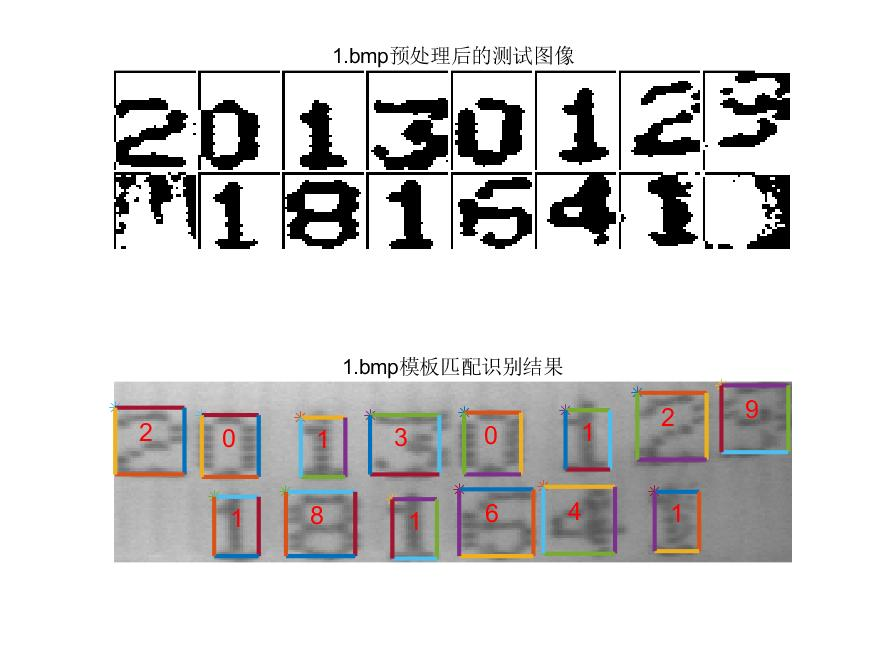
\includegraphics[width=\textwidth]{save1}
	\end{minipage}
	\begin{minipage}[t]{0.48\textwidth}
		\centering
		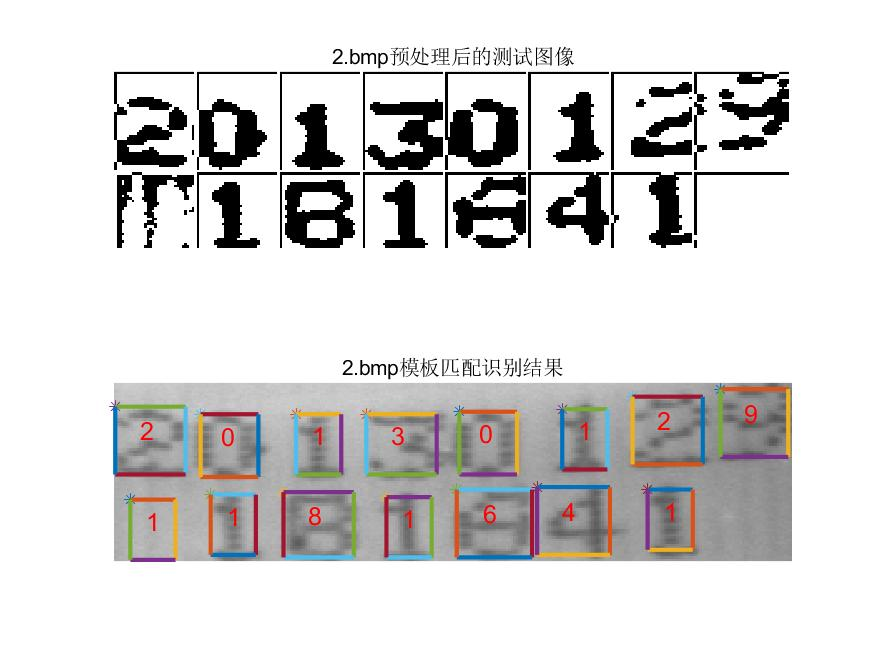
\includegraphics[width=\textwidth]{save2}
	\end{minipage}
	\begin{minipage}[t]{0.48\textwidth}
		\centering
		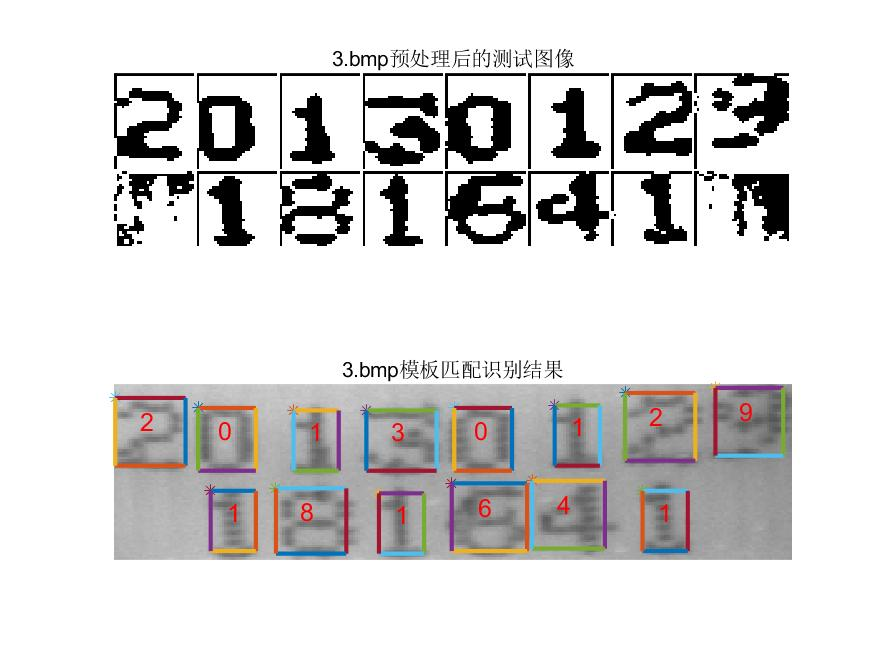
\includegraphics[width=\textwidth]{save3}
	\end{minipage}
	\begin{minipage}[t]{0.48\textwidth}
		\centering
		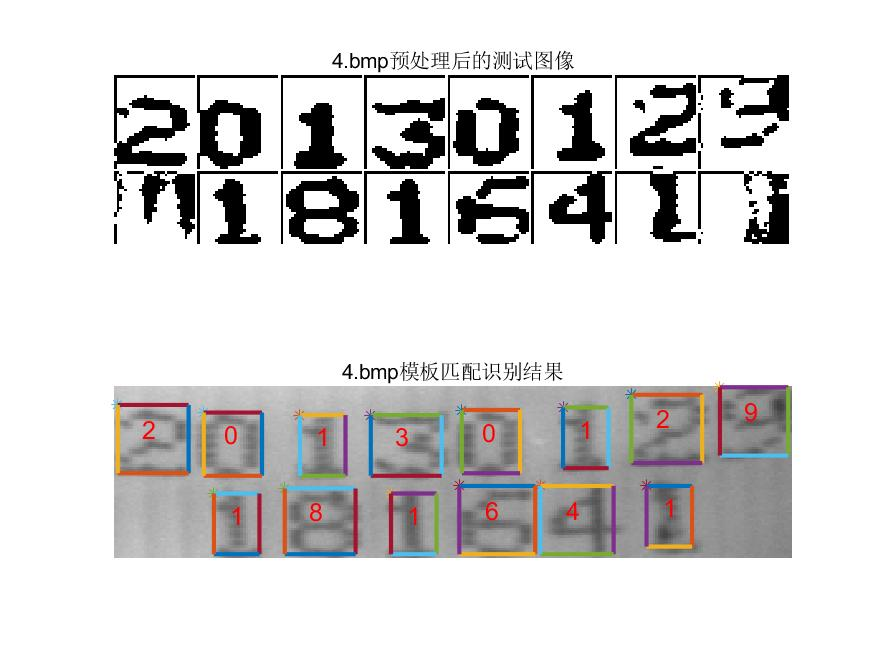
\includegraphics[width=\textwidth]{save4}
	\end{minipage}
	\begin{minipage}[t]{0.48\textwidth}
		\centering
		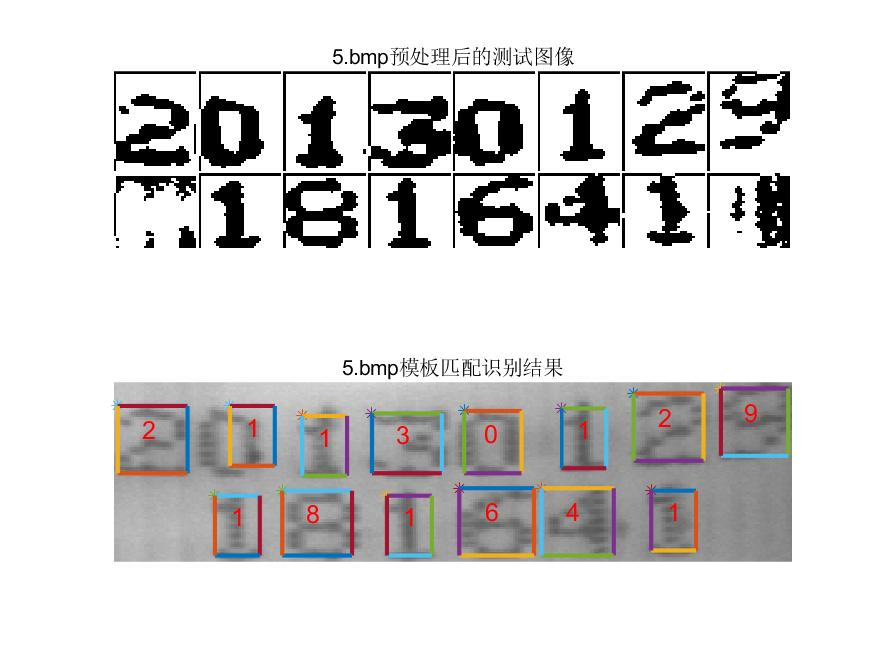
\includegraphics[width=\textwidth]{save5}
	\end{minipage}
	\begin{minipage}[t]{0.48\textwidth}
		\centering
		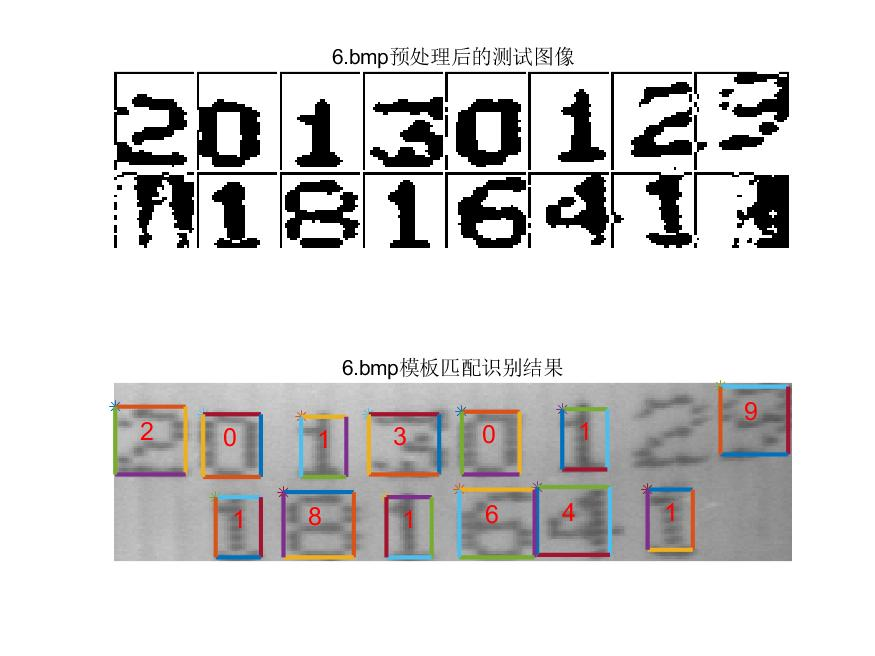
\includegraphics[width=\textwidth]{save6}
	\end{minipage}
	\caption{\label{hua1}采用滑动窗模板匹配的正常图片识别结果}
\end{figure}

\subsection{噪声图片识别结果}

首先对噪声图片进行第\ref{sec12}节介绍的预处理操作,然后再对其进行滑窗模板匹配操作,得到如图\ref{hua2}所示的识别结果。

\begin{figure}[!h]
	\centering
	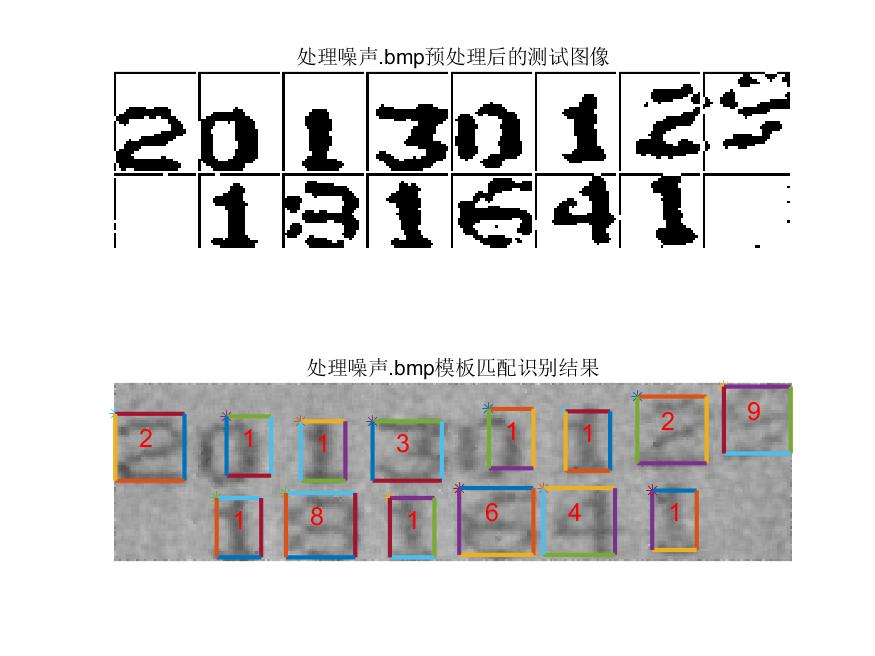
\includegraphics[width=\textwidth]{save8}
	\caption{\label{hua2}噪声图片识别结果}
\end{figure}
\begin{figure}[!h]
	\centering
	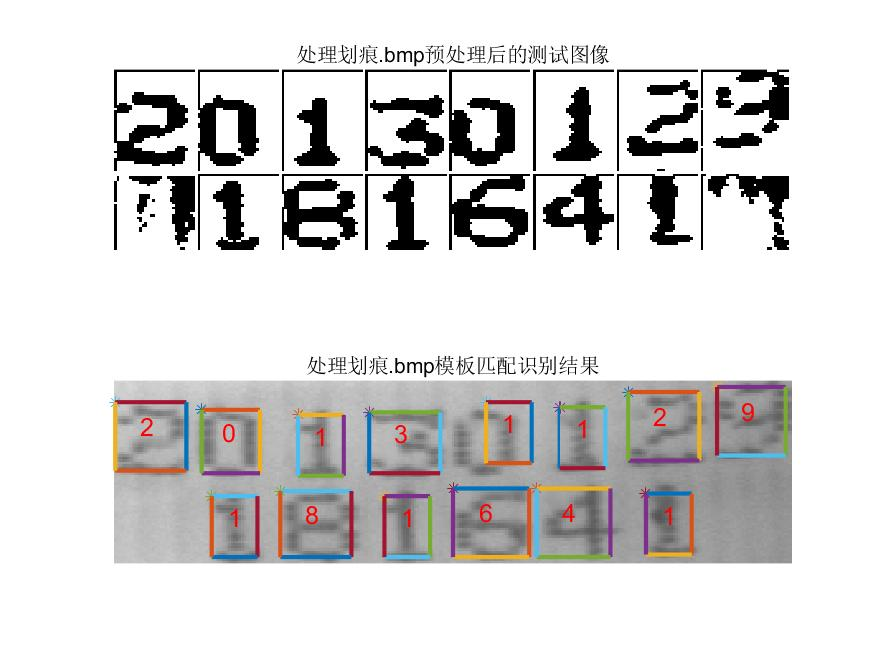
\includegraphics[width=\textwidth]{save7}
	\caption{\label{hua3}划痕图片识别结果}
\end{figure}

\subsection{划痕图片识别结果}

首先对划痕图片进行第\ref{sec13}节介绍的预处理操作,然后再对其进行滑窗模板匹配操作,得到如图\ref{hua3}所示的识别结果。

\subsection{结果总结}
我们总结了此种方法下各个字符的召回率和虚警率如表\ref{tab2}所示。从表中可以看出,基于滑窗的模板匹配主要出错的点是将0判别为1了,这是由于在滑动的过程中,模板先滑到了0的左边界,与1的相关系数较高,因此判别为1也不足为奇了。
\begin{table}[!htbp]
	\centering
	\caption{滑动窗匹配的数字字符识别结果统计}\label{tab2}%添加标题 设置标签
	\begin{tabular}{ccc}
		\toprule
		字符& 召回率TP& 虚警个数\\
		\midrule
		0& 13/16 & 0\\
		1& 40/40 & 4\\
		2& 15/16 & 0\\
		3& 8/8 & 0 \\
		4& 8/8 & 0 \\
		6& 8/8 & 0 \\
		8& 8/8 & 0 \\
		9& 8/8 & 0 \\
		\bottomrule
	\end{tabular}
	%\caption{这是一张三线表}\label{tab:aStrangeTable}  标题放在这里也是可以的
\end{table}

\section{多尺度模板匹配}
\label{sec3}
对于图像与模板不匹配的情况,我们不能直接使用图\ref{fig:1}所示的流程图进行模板匹配,我们需要对模板进行多尺度变换之后与测试图像进行匹配。算法流程图如图\ref{fig:2}所示。

\begin{figure}[!ht]
	\centering
	\begin{tikzpicture}
	\node (step1) [startstop] {滑动检测窗口};
	\node (step2) [startstop, below of=step1, yshift=-0.5cm] {用模板判断是否为目标};
	\node (step5) [startstop, right of=step2, xshift=3cm] {缩放模板};
	\node (step3) [startstop, below of=step2, yshift=-0.5cm] {对检测结果进行融合};
	\node (step4) [startstop, below of=step3, yshift=-0.5cm] {得到检测结果};
	
	\draw [arrow] (step1) -- (step2);
	\draw [arrow] (step2) -- (step3);
	\draw [arrow] (step3) -- (step4);
	\draw [arrow] (step3) -| (step5) |- (step1);
	\end{tikzpicture}
	\caption{\label{fig:2}基于滑动窗的多尺度模板匹配示意图}
\end{figure}

\begin{figure}[!h]
	\centering
	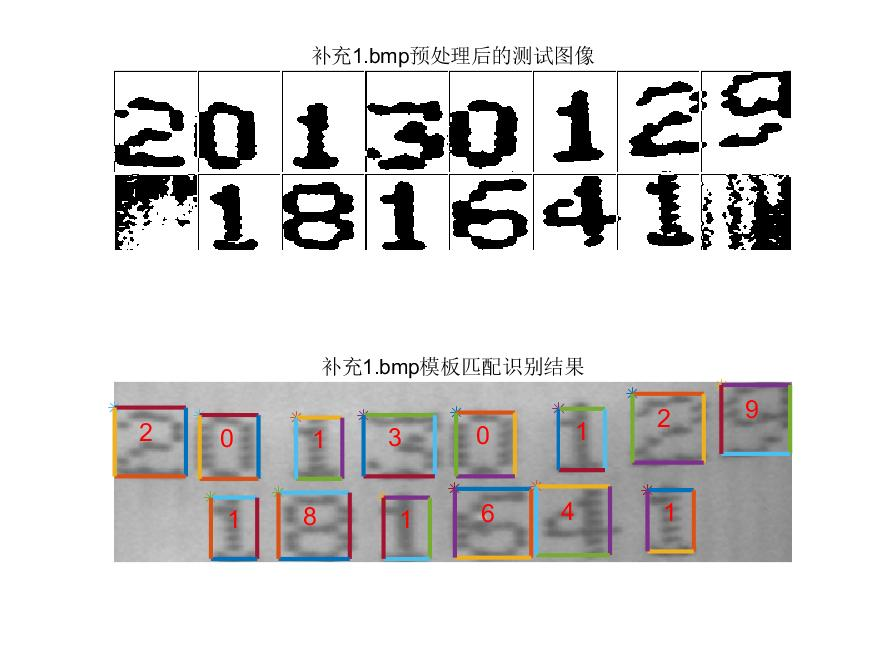
\includegraphics[width=\textwidth]{multi1}
	\caption{\label{buchong1}放大图片识别结果}
\end{figure}
\begin{figure}[!h]
	\centering
	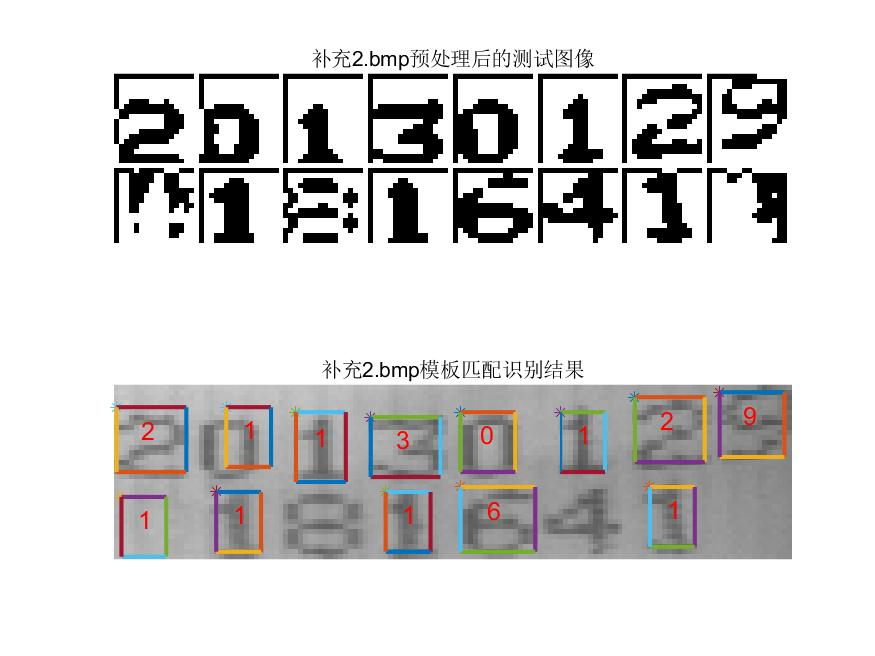
\includegraphics[width=\textwidth]{multi2}
	\caption{\label{buchong2}缩小图片识别结果}
\end{figure}

分别对补充1和补充2的图片首先进行预处理(去除光照影响、二值化等),然后分别将模板图片进行多尺度缩放,之后再与预处理之后的测试图片进行滑动相关,取结果最大的数字字符作为识别结果。如图\ref{buchong1}和图\ref{buchong2}所示,分别为放大的图片和缩小图片的识别结果,从图中可以看出,对于尺度增大的图片识别率为100\%,由此可以说明,使用多尺度的滑动窗模板匹配算法对放大的图片效果较好,但是对于尺度缩小的图片,有1个识别错误,2个未识别出来,原因在于将模板缩小尺度的过程中图片会有失真,因此导致检测效果不好。

\chapter{基于特征提取的模板匹配}
\label{sec4}
在本章,我们将首先对图像分块提取特征,最后将特征合并在一起用于匹配,同时,我们依然使用了上一章的图像预处理的方法,为的是使我们的识别更加准确。

%\section{特征设计}
首先,我们采用作业中提示的方式对图像分块进行特征提取。如图\ref{feat1}所示,将图像分块,每块逐行或者逐列统计黑像素点的个数作为局部特征,然后使用特征来进行模板匹配。对正常图片的识别结果如图\ref{feat2}所示,对噪声图片(使用了\ref{sec12}的处理算法)的识别结果如图\ref{feat3}所示,对划痕图片(使用了\ref{sec13}的处理算法)的的识别结果如图\ref{feat4}所示。
\begin{figure}[!h]
	\centering
	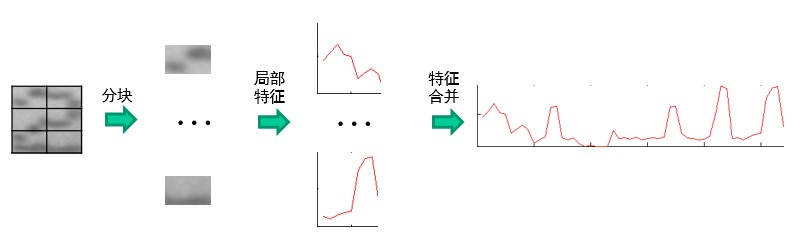
\includegraphics[width=\textwidth]{feat1}
	\caption{\label{feat1}图像分块计算特征}
\end{figure}

我们总结了此种方法下各个字符的召回率和虚警率如表\ref{tab3}所示。从表中可以看出,基于特征提取的数字字符识别结果相比于直接的滑动窗模板匹配算法识别率更高,并且滑动窗算法中0被误识别为1的现象在特征提取的算法中也避免了,这是由于局部统计信息时0的边缘位置与1的特征相差较大,因此避免了这种现象。同时,从结果图中我们可以看出。噪声图片和划痕图片的识别率均达到了100\%,说明我们在第一章中提出的预处理算法是比较强的。
\begin{table}[!htbp]
	\centering
	\caption{基于特征提取的数字字符识别结果统计}\label{tab3}%添加标题 设置标签
	\begin{tabular}{ccc}
		\toprule
		字符& 召回率TP& 虚警个数\\
		\midrule
		0& 16/16 & 0\\
		1& 40/40 & 0\\
		2& 16/16 & 0\\
		3& 8/8 & 0 \\
		4& 6/8 & 0 \\
		6& 8/8 & 0 \\
		8& 8/8 & 0 \\
		9& 8/8 & 1 \\
		\bottomrule
	\end{tabular}
	%\caption{这是一张三线表}\label{tab:aStrangeTable}  标题放在这里也是可以的
\end{table}

\begin{figure}[!h]
	\centering
	\begin{minipage}[t]{0.48\textwidth}
		\centering
		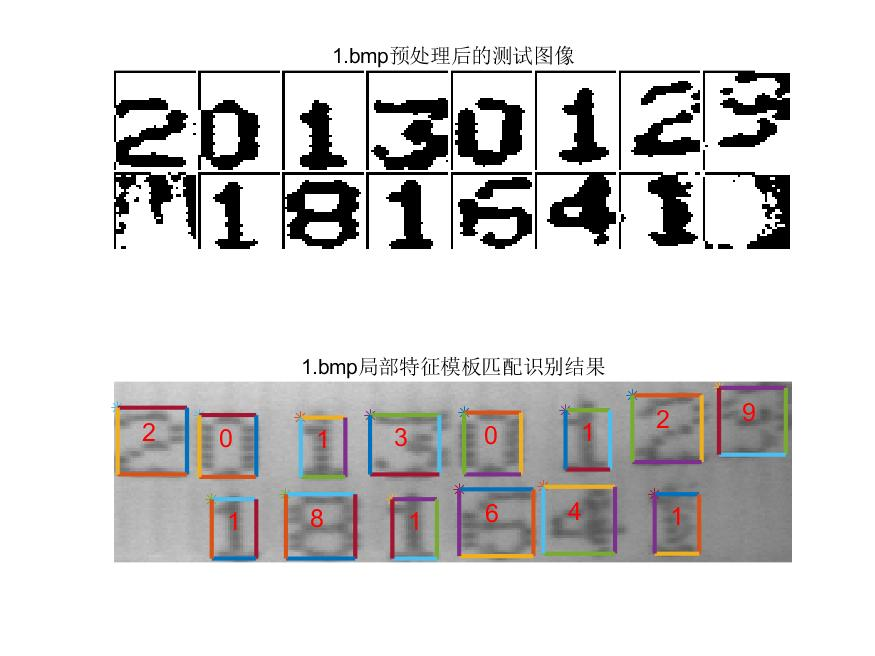
\includegraphics[width=\textwidth]{save21}
	\end{minipage}
	\begin{minipage}[t]{0.48\textwidth}
		\centering
		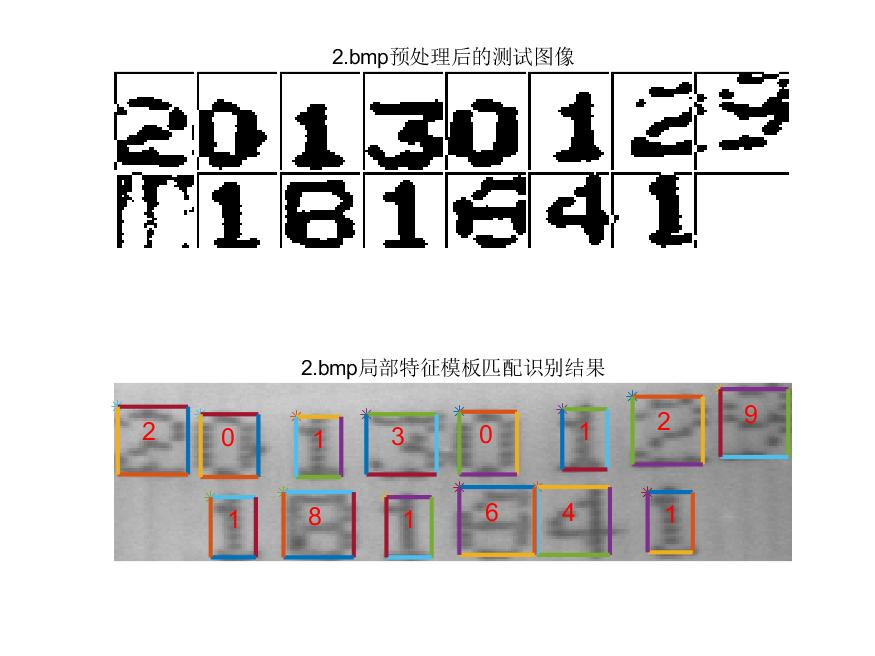
\includegraphics[width=\textwidth]{save22}
	\end{minipage}
	\begin{minipage}[t]{0.48\textwidth}
		\centering
		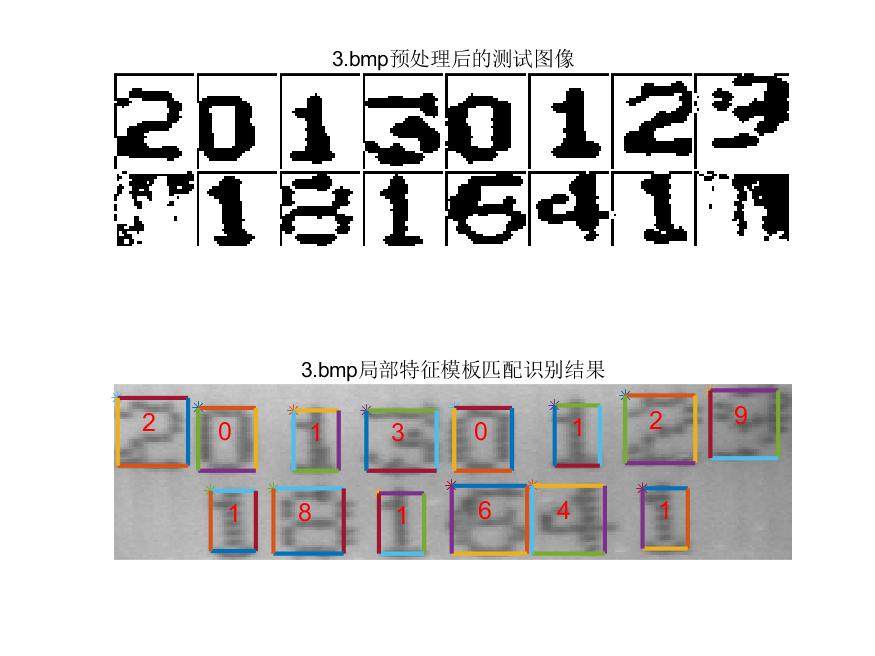
\includegraphics[width=\textwidth]{save23}
	\end{minipage}
	\begin{minipage}[t]{0.48\textwidth}
		\centering
		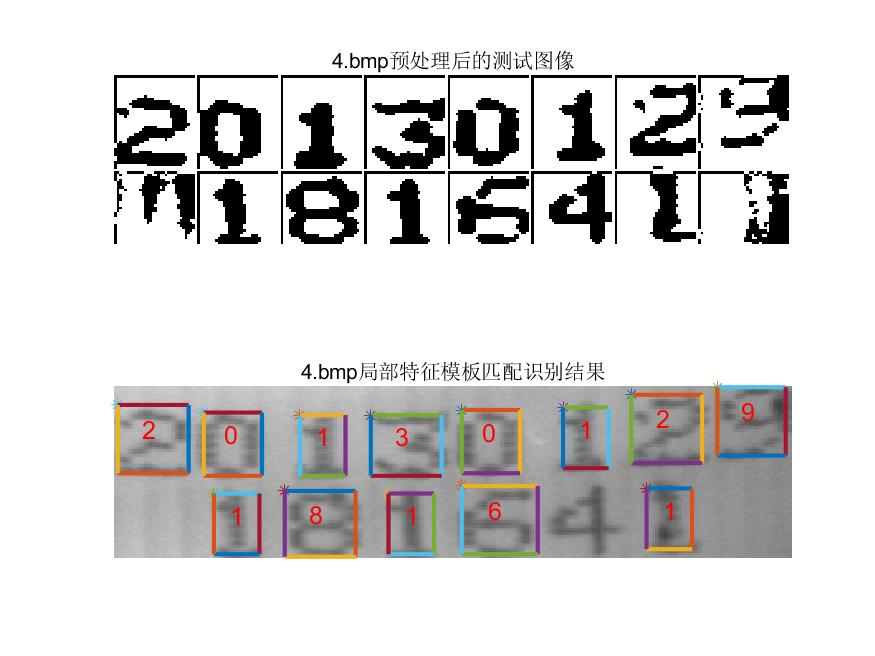
\includegraphics[width=\textwidth]{save24}
	\end{minipage}
	\begin{minipage}[t]{0.48\textwidth}
		\centering
		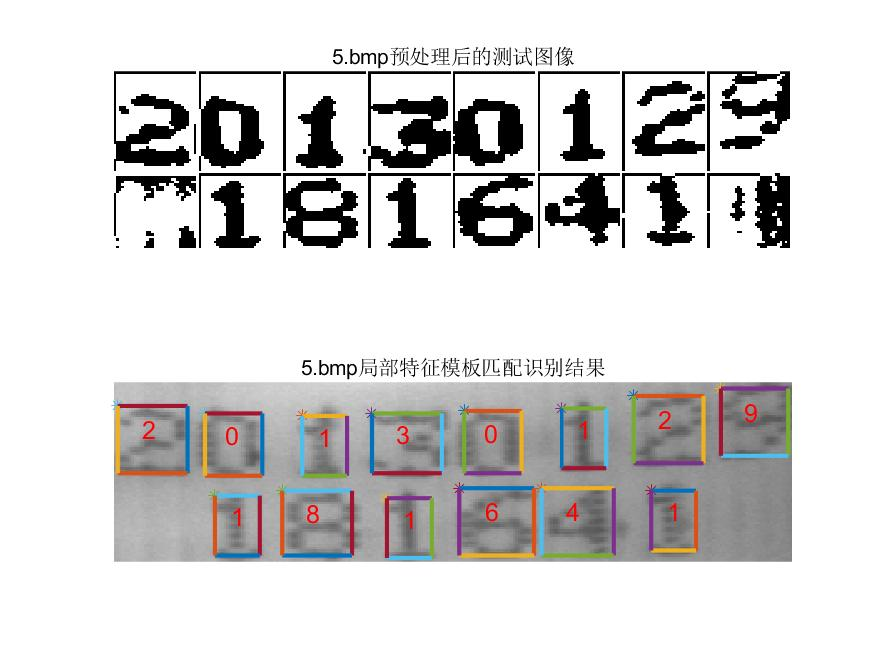
\includegraphics[width=\textwidth]{save25}
	\end{minipage}
	\begin{minipage}[t]{0.48\textwidth}
		\centering
		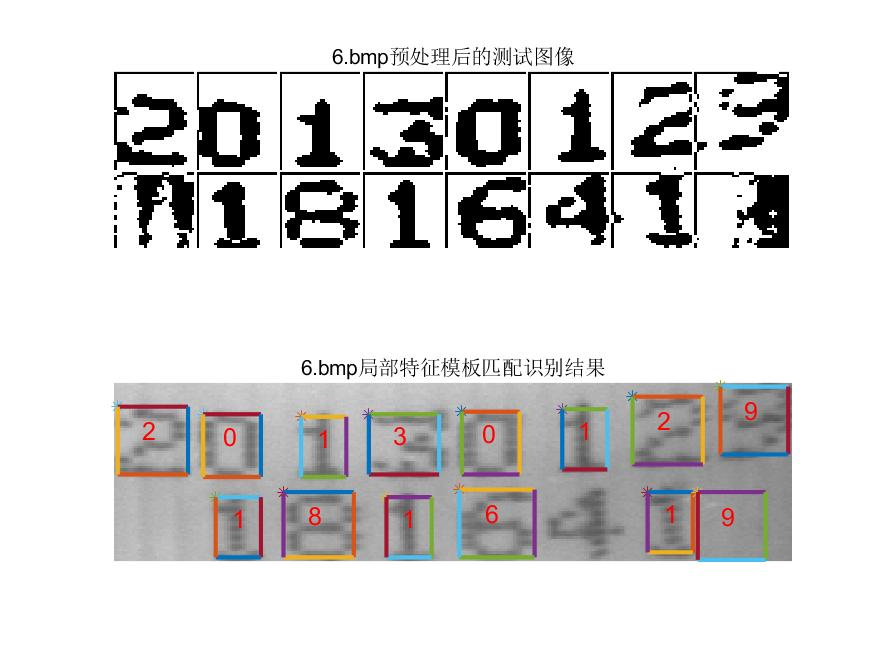
\includegraphics[width=\textwidth]{save26}
	\end{minipage}
	\caption{\label{feat2}采用特征提取模板匹配的正常图片识别结果}
\end{figure}

\begin{figure}[!h]
	\centering
	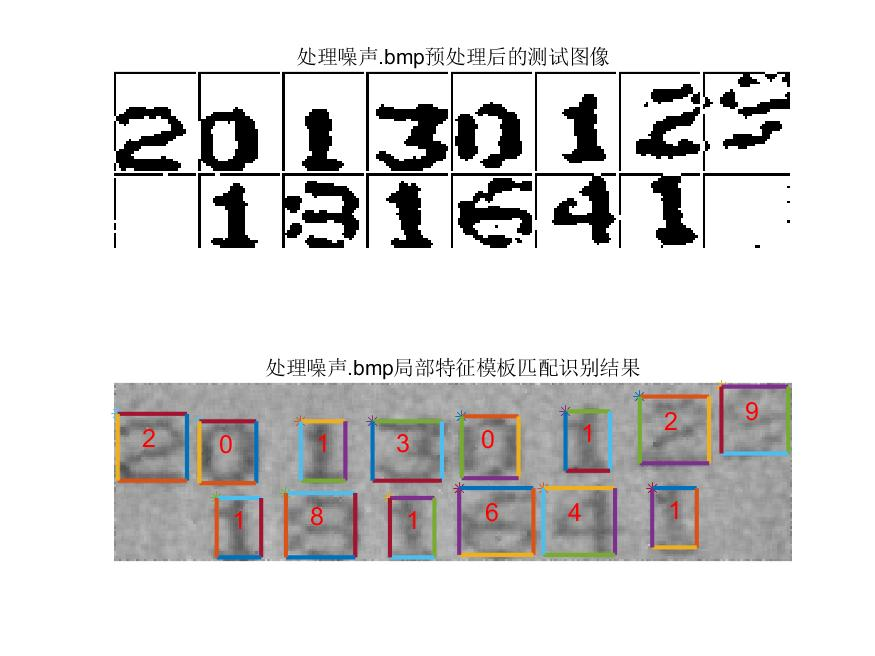
\includegraphics[width=\textwidth]{save28}
	\caption{\label{feat3}采用特征提取模板匹配的噪声图片识别结果}
\end{figure}
\begin{figure}[!h]
	\centering
	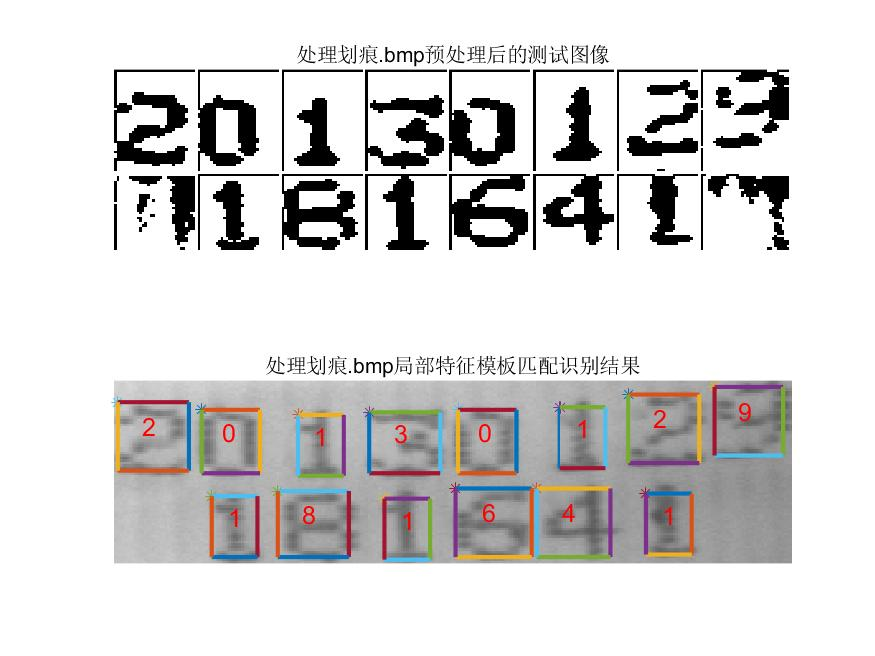
\includegraphics[width=\textwidth]{save27}
	\caption{\label{feat4}采用特征提取模板匹配的划痕图片识别结果}
\end{figure}

\chapter{总结}
本次大作业使用模板匹配的方式对数字字符进行识别,我们主要采用了基于分割的模板匹配、基于滑动窗的模板匹配以及基于特征提取的模板匹配三种算法,并且使用了一些数字图像处理的算法对图像进行了一系列的预处理。

对于训练集的模板图片,我们采用二值化的方式将其转换为二值图片。对于噪声图片我们采用了维纳滤波的方式去除噪声,然后再去除光照影响,最后再二值化用于模板匹配。对于划痕图片,我们首先使用阈值将划痕检测出来,然后将其像素值置为NaN,然后采用插值的算法填充缺失值,最后再去除光照影响、二值化。从实验结果来看,我们对于噪声图片和划痕图片的预处理是非常成功的,在基于特征提取的模板匹配和基于分割的模板匹配中均达到了100\%的正确率。

对于基于分割的模板匹配算法,对于特定的图片算法实现简单直观,但是如果给出的测试集图片结构发生变化便需要重新修改代码重新分割;对于滑动窗的模板匹配算法,主要问题是把0识别为1;而基于特征提取的模板匹配算法较好的解决了0误识别为1的现象。所以三种算法中,基于特征提取的算法更好。特征提取的方法有很多种,例如SIFT特征、HoG特征等,甚至我们可以使用神经网络来提取特征再进行模板匹配,但是这样计算复杂度会增加很多,在本次大作业中没有进行尝试。

对于不同尺度的图片,我们主要采用了多尺度模板匹配的算法,对于放大的图片识别性能较好,对于缩小的图片识别性能欠佳。我们可以通过更改不同尺度下匹配结果的阈值来更加精确的调节。

最后,通过本次作业学习了模板匹配的方法在模式识别中的应用,同时复习了数字图像处理的相关知识。

\chapter{文件说明}
“code/”文件夹中放置的是本次作业用到的代码文件,“train/”文件夹中放置的提供的训练集模板文件,“test/”文件夹下放置的是提供的测试集文件以及\textbf{预处理之后的划痕、噪声文件},“train\_bw/”文件夹下放置的是预处理之后的模板文件。以下将对“code/”文件夹下的主要代码进行说明:
\begin{itemize}
	\item \textbf{main.m}:使用基于分割的模板匹配的主函数,直接执行即可得到第\ref{sec1}节的结果;
	\item \textbf{slideMain.m}:使用基于滑动窗的模板匹配的主函数,直接执行即可得到第\ref{sec2}节的结果;
	\item \textbf{multiscaleMain.m}:对缩小和放大的图片进行多尺度模板匹配的主函数,直接执行即可得到第\ref{sec3}节的结果;
	\item \textbf{slideMainFeature.m}:使用基于特征提取的模板匹配的主函数,直接执行即可得到第\ref{sec4}章的结果;
	\item processNoisy.m:对噪声图片进行预处理的代码,并且绘制了处理前后的对比图,并将处理后的图片保存在“test/”文件夹下;
	\item processScratch.m:使用腐蚀膨胀的算法对划痕图片预处理的代码,实验效果一般;
	\item processScratchImage.m:使用第一章提到的算法对划痕图片进行预处理的代码,实验效果较好;
	\item inpaintn.m:使用插值算法对图像缺失值进行填补的算法代码,使用了Matlab开源包里的内容;
	\item processTrain.m:绘制训练集模板图片预处理前后的对比图;
	\item predictNormalImage.m:使用基于分割的模板匹配算法对正常图片识别的函数;
	\item predictNoisyImage.m:使用基于分割的模板匹配算法对噪声图片识别的函数;
	\item predictScrachImage.m:使用基于分割的模板匹配算法对划痕图片识别的函数;
	\item predictNum.m:使用基于分割的模板匹配算法中预测数字的函数;
\end{itemize}
\end{document}